% Slides accompanying "Learn RISC-V CPU Implementation and BSV" book
% Copyright (c) 2024 Rishiyur S. Nikhil, All Rights Reserved

% -*- mode: fundamental -*-

% Slides accompanying "Learn RISC-V CPU Implementation and BSV" book
% Copyright (c) 2024 Rishiyur S. Nikhil, All Rights Reserved

% This is a preamble shared by all the slide decks

\documentclass[10pt, aspectratio=169]{beamer}

% \documentclass[17pt]{beamer}

% Avail. font sizes: 8pt, 9pt, 10pt, 11pt, 12pt, 14pt, 17pt, 20pt.
% Default font size is 11pt (= 22pt in full screen mode).

\usepackage{verbatim}
\usepackage{fancyvrb}
\usepackage{listings}

% ================================================================
% Themes

\usetheme{Madrid}          % Line at bottom: Author (affiliation), OptTitle, Conf, page 

% \usetheme{Copenhagen}    % Same as Madrid except bottom line: Author, OptTitle

% \usetheme{Berkeley}    % Takes up 1-inch border on left and top

% ----------------
% colorthemes
% (default), beaver, beetle, seahorse, wolverine

\usecolortheme{seahorse}

% ================================================================
% Customization: show table of contents before each section
% Use \AtBeginSubsection    to show before each subsection

% \AtBeginSection[]
% {
%   \begin{frame}
%     \frametitle{Table of Contents}
%     \tableofcontents[currentsection]
%   \end{frame}
% }

% ================================================================

% ----------------
% The bsc compiler and BSV language
\newcommand{\bsc}{\emph{bsc}}
\newcommand{\BSV}{\bf{BSV}}
% ----------------
% ITALICISE WORDS
\newcommand{\ie}{\emph{i.e.,}}
\newcommand{\eg}{\emph{e.g.,}}
\newcommand{\Eg}{\emph{E.g.,}}
\newcommand{\etc}{\emph{etc.}}
\newcommand{\via}{\emph{via}}
\newcommand{\vs}{\emph{vs.}}

% ----------------
% EMPTY BOXES OF VARIOUS WIDTHS, FOR INDENTATION

\newcommand{\hm}{\hspace*{1em}}
\newcommand{\hmm}{\hspace*{2em}}
\newcommand{\hmmm}{\hspace*{3em}}
\newcommand{\hmmmm}{\hspace*{4em}}

% ----------------
% Convenient widths

\newlength{\hlessmm}
\setlength{\hlessmm}{\textwidth}
\addtolength{\hlessmm}{-2em}

\newlength{\hlessmmm}
\setlength{\hlessmmm}{\textwidth}
\addtolength{\hlessmmm}{-3em}

\newlength{\hlessmmmm}
\setlength{\hlessmmmm}{\textwidth}
\addtolength{\hlessmmmm}{-4em}

% ================================================================
% Title page

\title[Learn CPU design \& BSV]{Learn RISC-V CPU Implementation and BSV}

\subtitle{(BSV: a High-Level Hardware Design Language)}

\author[{\copyright} R.S.Nikhil]{Rishiyur S.~Nikhil}
% \institute{Bluespec, Inc.}

% Date is set differently in each slide deck

% \logo{
\includegraphics[height=0.6cm]{../Figures/Bluespec_Logo_2022-10}}

% End of preamble
% ****************************************************************


\date{L13: {\BSV}: Rules and their semantics}

% ****************************************************************

\begin{document}

% ================================================================

\begin{frame}
 \titlepage

 \begin{center}
  
\includegraphics[height=1cm]{Bluespec_Logo_2022-10}
 \end{center}

\end{frame}

% ================================================================

% -*- mode: fundamental -*-

% ================================================================

\begin{frame}[fragile]
\frametitle{Reminders}

\footnotesize

Please git clone: \url{https://github.com/rsnikhil/Learn_Bluespec_and_RISCV_Design} \\
(git pull for latest version).  Repsitory structure:

\vspace{1ex}

\begin{minipage}{0.5\textwidth}\scriptsize
\begin{Verbatim}[frame=single, numbers=left]
    ./Book_BLang_RISCV.pdf
      Slides/
          Slides_01_Intro.pdf
          Slides_02_ISA.pdf
          ...
      Exercises/
          Ex-03-A-Hello-World/
          Ex-03-B-Top-and-DUT/
          ...
      Code/
          src_Top/
          src_Drum/
          src_Fife/
          src_Common/
          ...
      Doc/Installing_bsc_Verilator_etc.{adoc,html}
\end{Verbatim}
\end{minipage}
\hm
\begin{minipage}{0.45\textwidth}
\begin{itemize}

 \item Slides and Exercise are numbered in sync with book Chapter numbers.

 \item For Exercises, please see Appendix E of the book.  Some (not
       all) exercises have associated code in the {\tt Exercises/}
       directory.

\end{itemize}
\end{minipage}

\vspace{2ex}

To compile and run the code for exercises, Drum and Fife, please make sure you have installed:

\begin{itemize}

 \item \emph{bsc} compiler (see \url{https://github.com/B-Lang-org/bsc})

 \item Verilator compiler (see \url{https://www.verilator.org/})
\end{itemize}

\footnotesize

\end{frame}

% ================================================================

\begin{frame}
\frametitle{Chapter Roadmap}

\footnotesize

\begin{center}
\frame{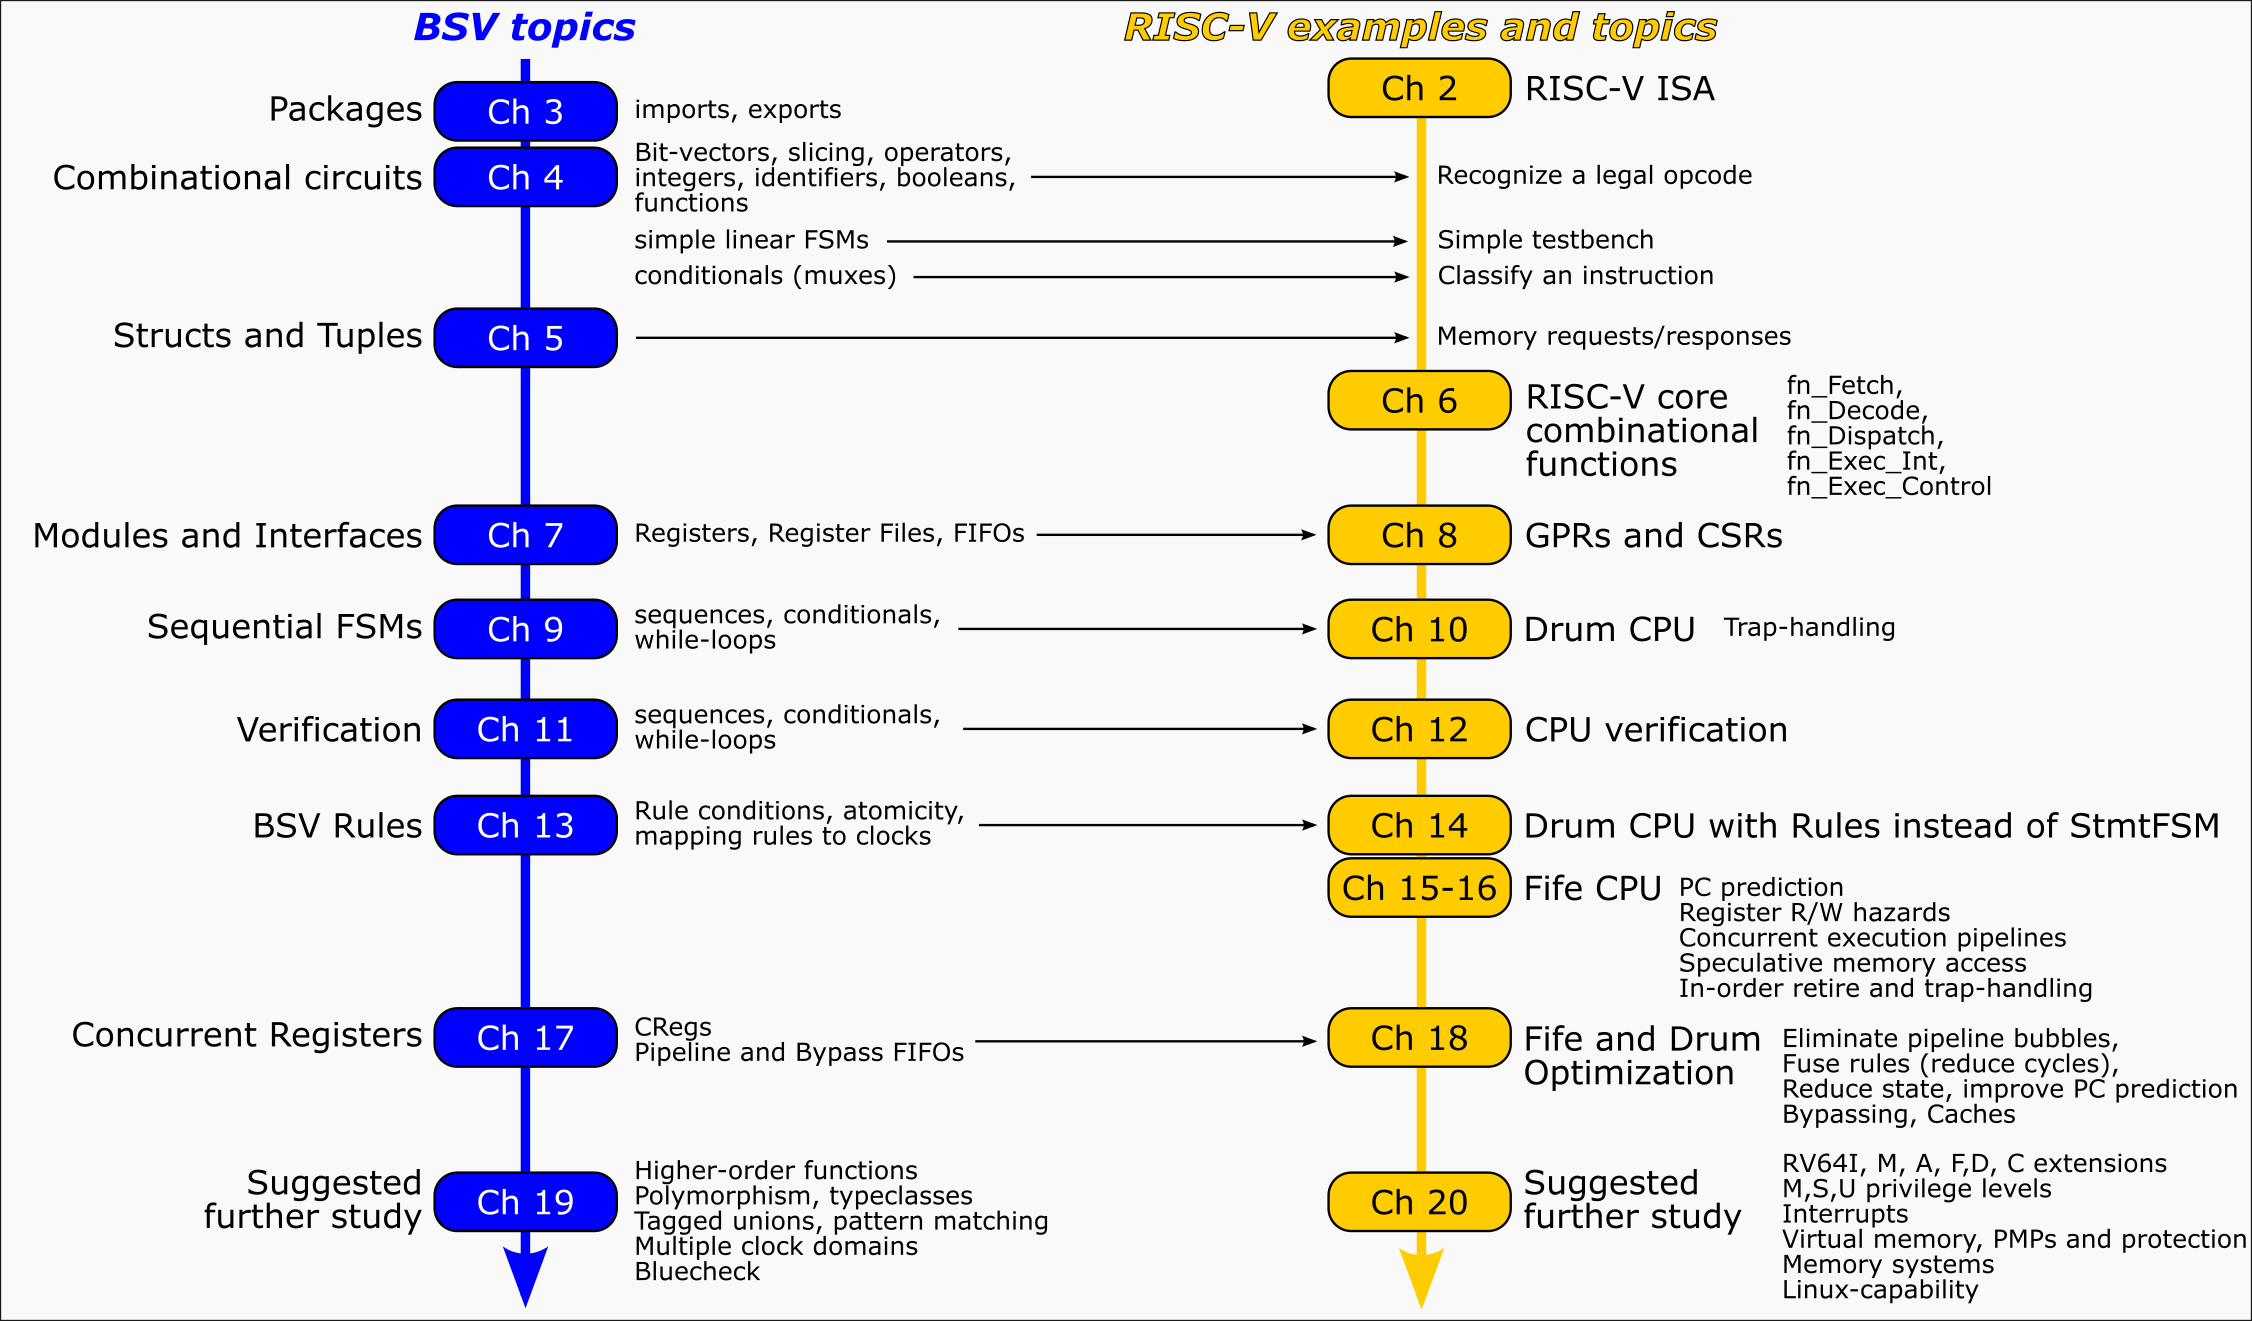
\includegraphics[height=0.825\textheight]{Fig_Chapter_Roadmap}}
\end{center}

\end{frame}

% ================================================================


% ================================================================

\begin{frame}
\frametitle{Flow of information between stages in Drum and Fife}

\footnotesize

\begin{center}
 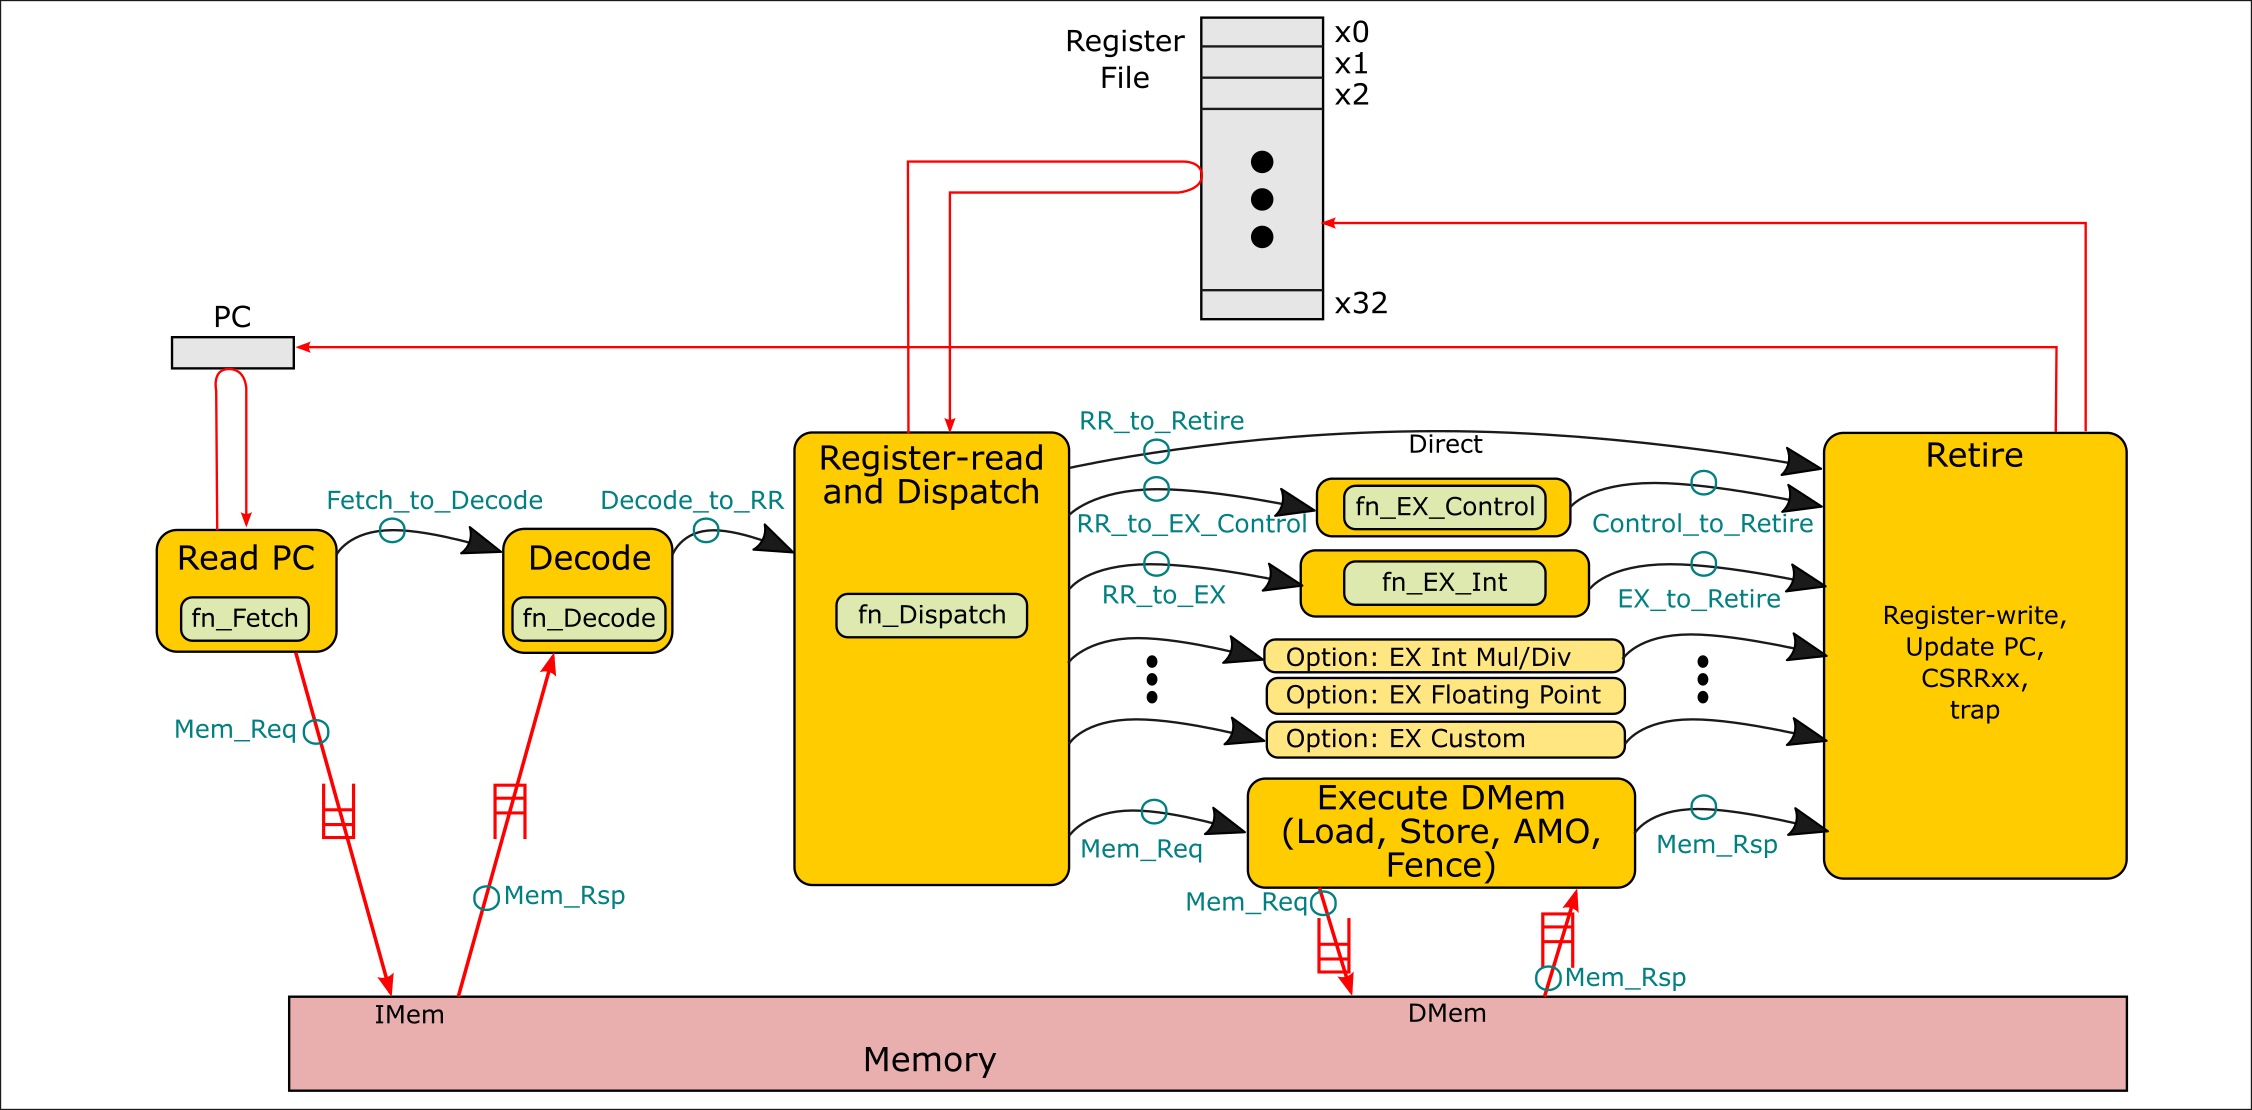
\includegraphics[height=0.6\textheight]{Fig_Instr_Exec_w_structs}
\end{center}

\end{frame}

% ================================================================

\begin{frame}
\frametitle{Table of Contents}

\tableofcontents

\end{frame}

% ****************************************************************

\section{{\BSV}: Rules: Introduction}

\begin{frame}

\begin{center}
  {\LARGE Rules: Introduction}
\end{center}

\end{frame}

% ================================================================

\begin{frame}[fragile]
\frametitle{Rules: the fundamental behavioral construct in {\BSV}}

\footnotesize

{\large ``\emph{Rules}'' are the fundamental constructs in {\BSV}
 to specify dynamic behavior.}

\vspace{4ex}

A {\tt rule}-{\tt endrule} construct appears in the body of a {\BSV} modules.

\vspace{1ex}

It represents a combinational circuit that typically invokes methods
in interfaces of other modules.

\vspace{1ex}

An interface method, in turn, is simply a ``mini-rule'' that is
semantically a part of a rule or interface method from which it is
invoked.

\vspace{1ex}

Thus, a rule consists of a {\tt rule}-{\tt endrule} construct plus
every method it invokes, plus every method that those methods invoke,
and so on.  Thus, a rule can observe and update state in several modules.

\PAUSE{\vspace{4ex}}

The \emph{functionality} of rules (semantics, ``what does it do?'')
can be understood in two incremental steps:

\begin{itemize}

 \item Semantics of a rule in isolation

 \item Semantics of the collection of rules in a {\BSV} program

\end{itemize}

\PAUSE{\vspace{4ex}}

The \emph{performance} of rules (how long does a computation take?)
can be understood by understanding how rules are mapped to clocks.

\end{frame}

% ================================================================

\begin{frame}[fragile]
\frametitle{Rules: Syntax, and data types for the two components}

\footnotesize

\begin{center}
 \includegraphics[width=6in,angle=0]{Fig_Rule_Structure}
\end{center}

\vspace{5ex}

A rule body is an implicit {\tt action}-{\tt endaction} block; it can
contain several sub-actions and identifier bindings.

\vspace{1ex}

\end{frame}

% ================================================================

\begin{frame}[fragile]
\frametitle{Rules: Implicit and overall condition}

\footnotesize

\begin{itemize}

\item Both the rule condition and the body may invoke interface methods of
      other modules.

\item Each method has an ``implicit condition'' (type {\tt Bool}; READY signal in hardware)
      indicating whether the method is currently enabled or not.

      {\Eg} for a standard FIFO $f$ , the $f${\tt .first} and $f${\tt
      .deq} methods have implicit conditions that are true only when
      the FIFO is non-empty.

\item A value-method like $f${\tt .first}, being
      pure (not {\tt Action} or {\tt ActionValue}), may be invoked
      both in rule conditions and in rule bodies.

\item An {\tt Action} or {\tt ActionValue}  method like $f${\tt .deq} can
      never be invoked in a rule condition, only in a rule body.

\end{itemize}

\vspace{5ex}

The overall rule condition, also known as its ``CAN\_FIRE'' condition,
is a conjunction (AND) of the rule’s explicit condition and implicit
conditions of any invoked methods, whether those methods are in the
rule condition or in the rule body.

\vspace{1ex}

For example, if a rule invokes $f${\tt .first} or $f${\tt .deq}, the
implicit condition of those methods become part of the CAN\_FIRE
condition of the rule.

\end{frame}

% ****************************************************************

\section{Semantics of a rule in isolation}

\begin{frame}

\begin{center}
  {\LARGE Semantics of a rule in isolation}
\end{center}

\end{frame}

% ================================================================

\begin{frame}[fragile]
\frametitle{Semantics of a rule in isolation}

\footnotesize

Each rule can be viewed as a pure function (therefore, a combinational
circuit) whose inputs come from various methods and which produces
outputs for various {\tt Action} and {\tt ActionValue} methods.

\vspace{5ex}

Each {\tt Action} or {\tt ActionValue} method has an implicit boolean
ENABLE argument (separate from its normal arguments and result).  An
{\tt Action} or {\tt ActionValue} method
\emph{performs} its action only when its ENABLE argument is asserted.

\end{frame}

% ================================================================

\begin{frame}[fragile]
\frametitle{Semantics of a rule in isolation}

\label{isolated_rule_semantics}

\footnotesize

\begin{minipage}{0.35\textwidth}
Example: the diagram below illustrates the function represented by this rule.
\end{minipage}
\hm
\begin{minipage}{0.6\textwidth}
\begin{Verbatim}[frame=single]
   rule rl_compute ((y != 0) && got_x && (f.first == 3));
    if (y [0] == 1) w <= w + x;
    x <= x << 1;
    g.enq (w * f.first);
   endrule
\end{Verbatim}
\end{minipage}

\begin{center}
 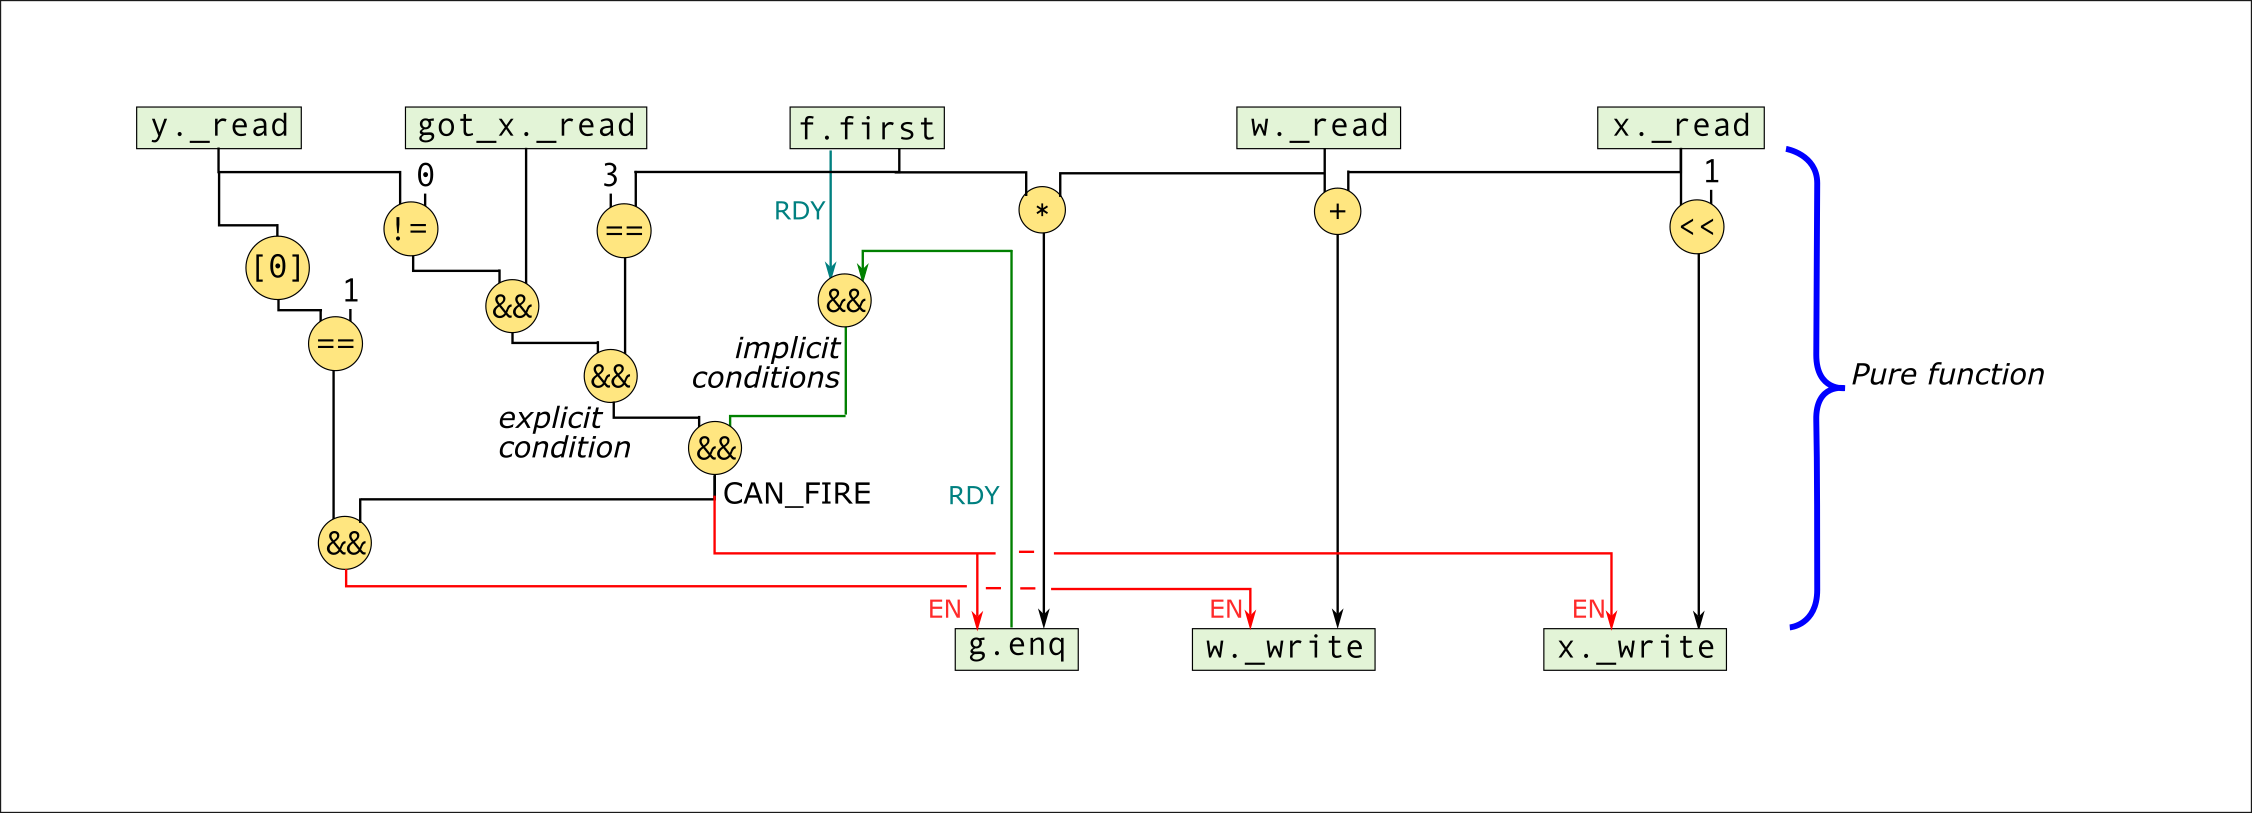
\includegraphics[width=0.85\textwidth]{Fig_Rule_Actions_1}

 This is just a functional illustration; we will see shortly that this
 maps straightforwardly into hardware.
\end{center}


\end{frame}

% ================================================================

\begin{frame}[fragile]
\frametitle{Recapping some properties of rules}

\footnotesize

\begin{itemize}

 \item All {\tt Action}s in a rule are
       performed \emph{simultaneously}, no matter what textual order
       they may appear in the rule body.  We also say that the actions
       all occur \emph{in parallel}.

 \item All {\tt Action}s in a rule are performed
       \emph{instantaneously}.

 \item Explicit rule conditions and method implicit conditions are
       combined to determine whether the rule executes at all.

 \item Some actions in a rule may be further restricted by
       if-then-else conditions in the rule.

\end{itemize}

       
\vspace{5ex}

Terminology: when a rule executes, we also say that the rule \emph{fires}.

\end{frame}

% ================================================================

\begin{frame}[fragile]
\frametitle{Hardware representation of a rule in isolation}

\label{Slide_HW_representation_of_a_rule}

\footnotesize

The semantic view of a rule in Slide~\ref{isolated_rule_semantics}
maps straightforwardly into hardware.

\vspace{1ex}

(Green signals are READY signals; Red signals are ENABLE signals.)

\vspace{4ex}

\begin{center}
 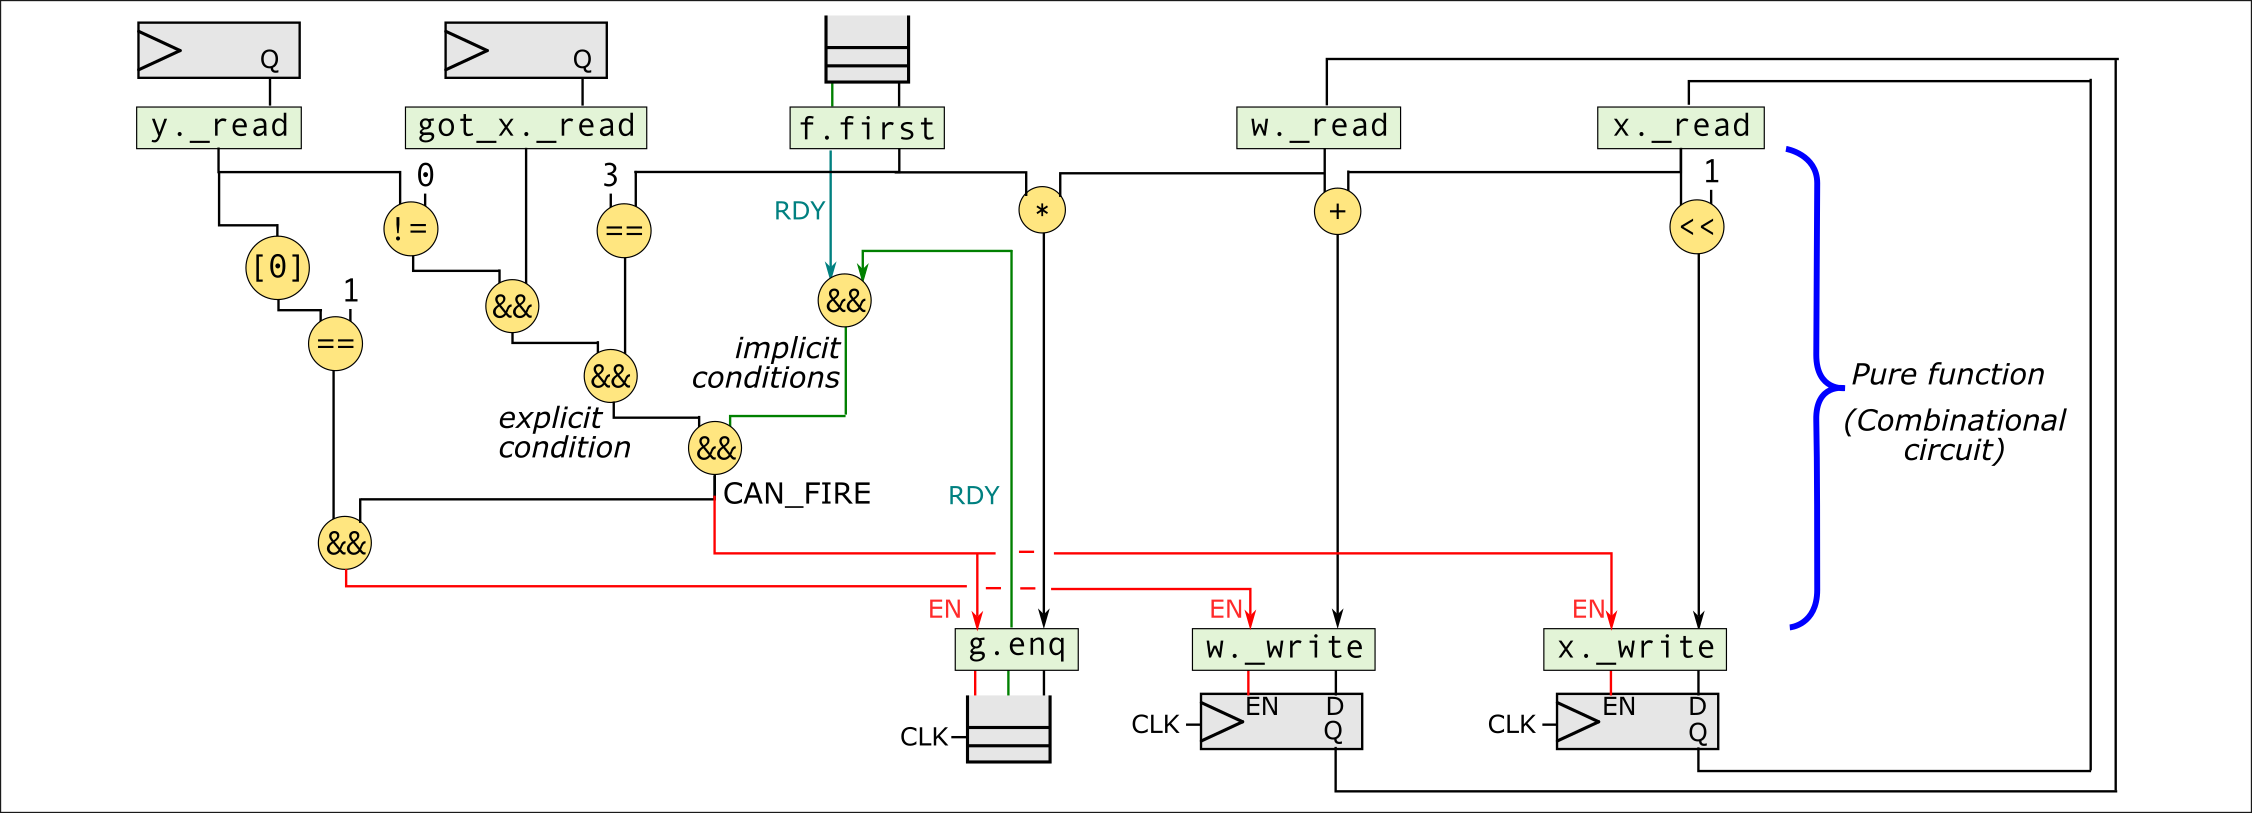
\includegraphics[width=\textwidth]{Fig_Rule_Actions_1_2}
\end{center}

\end{frame}

% ================================================================

\begin{frame}
\frametitle{\EmojiExercise \hmm Exercise break}

Please see Book Appendix E, Section Ex-13-A-Simultaneous-Actions.

\end{frame}

% ================================================================

\begin{frame}[fragile]
\frametitle{Note: a rule firing cannot perform the same action more than once}

\footnotesize

The following example illustrates some absurdities:

\vspace{2ex}

\begin{minipage}{0.5\textwidth}
\begin{Verbatim}[frame=single]
    rule rl_foo (...);
       x <= 2;           x <= 3;
       f.enq (2);        f.enq (3);
       g.deq;            g.deq;
    endrule
\end{Verbatim}
\end{minipage}
\hm
\begin{minipage}{0.45\textwidth}
We cannot, in the same instant:
\begin{itemize}
 \item write into a register more than once;
 \item enqueue into a FIFO more than once;
 \item dequeue from a FIFO more than once
\end{itemize}
\end{minipage}

\vspace{5ex}

The \emph{bsc} compiler will flag such errors in a program with a
message like:

\vspace{1ex}

\hmmm ``Cannot compose actions in parallel''

\end{frame}

% ****************************************************************

\section{Semantics of a collection of rules}

\begin{frame}

\begin{center}
  {\LARGE Semantics of a collection of rules}
\end{center}

\end{frame}

% ================================================================

\begin{frame}[fragile]
\frametitle{Semantics of a collection of rules}

\footnotesize

The semantics of a collection of {\BSV} rules is: execute one-rule-at-a-time:

\begin{center}
 \fbox{
  \begin{minipage}{0.8\textwidth}
   while True \\
   \hmm Choose \emph{any} rule whose CAN\_FIRE is true \\
   \hmm \hmm Perform the actions in that rule's body \\

   \hmm \hmm {\scriptsize (this will likely modify state, affecting enabled
             CAN\_FIRE signals for the next iteration)}
  \end{minipage}
 }
\end{center}

By definition (because one-at-a-time):
\begin{itemize}

 \item The state observed (reads) by a rule cannot be changing during rule execution

 \item The state updates (writes) by a rule cannot be observed by any
       other rule while it is changing.
\end{itemize}

\begin{center}
\fbox{We also say: rules are \emph{atomic}}
\end{center}

\PAUSE{\vspace{2ex}}

{\BSV} \emph{implementations} may (and do) execute rules concurrently and in parallel, \\
as long as it remains \emph{consistent} with one-rule-at-a-time (atomic) semantics.

\vspace{1ex}

Analogies:
\fbox{
\begin{minipage}{0.8\textwidth}\tiny
\begin{itemize}
 \item RISC-V Instruction Semantics are one-instruction-at-a-time (instructions are atomic). \\
       This is the refence standard for ``correct'' behavior.

       RISC-V \emph{implementations} may (and do) re-order
       instructions and execute multiple instructions at a time
       (pipelining, superscalarity).

 \item C/C++ semantics are one-statement-at-a-time (statements are atomic). \\
       This is the refence standard for ``correct'' behavior.

       C/C++ \emph{implementations} may (and do) re-order and
       interleave instructions for different statements.
\end{itemize}
\end{minipage}}

\end{frame}

% ================================================================

\begin{frame}[fragile]
\frametitle{Semantics of rules: two sometimes surprising observations}

\footnotesize

NOTE: \fbox{
\begin{minipage}{0.9\textwidth}

The semantics of rules is non-deterministic---if CAN\_FIRE is true for
several rules, we can choose any one.  This is common in formal
specification languages for concurrent systems, allowing reasoning
about correctness under \emph{all} possible choices (different
implementations may make different choices, statically or
dynamically).

\vspace{1ex}

The \emph{bsc} compiler makes particular choices, resulting in deterministic hardware.

\end{minipage}}

\vspace*{5ex}

NOTE: \fbox{
\begin{minipage}{0.9\textwidth}

Although {\BSV} is a hardware design language (HDL), functional
correctness of a {\BSV} program only appeals to rule-at-a-time
semantics, without any reference to clocks.

\vspace{1ex}

(Just as the functional correctness of a RISC-V implementation only
appeals to one-instruction-at-a-time RISC-V ISA semantics, without any
reference to clocks or cycles.)

\vspace{1ex}

It is only for reasoning about performance (``how fast is the
implementation?'') that we need to appeal to clocks, cycles and
implementation details.

\end{minipage}}

\end{frame}

% ****************************************************************

\section{Implementing rules in clocked digital hardware}

\begin{frame}

\begin{center}
  {\LARGE Implementing rules in clocked digital hardware}
\end{center}

\end{frame}

% ================================================================

\begin{frame}[fragile]
\frametitle{Implementing rules in clocked digital hardware}

\footnotesize

Rule semantics provide only an abstract view of time: one rule
executes \emph{before} or \emph{after} another, and we cannot ascribe
any real-time measure (seconds, microseconds, nanoseconds) to rule
executions.

\vspace{5ex}

Digital hardware is driven by a clock signal with a specific time-period:

\begin{center}
 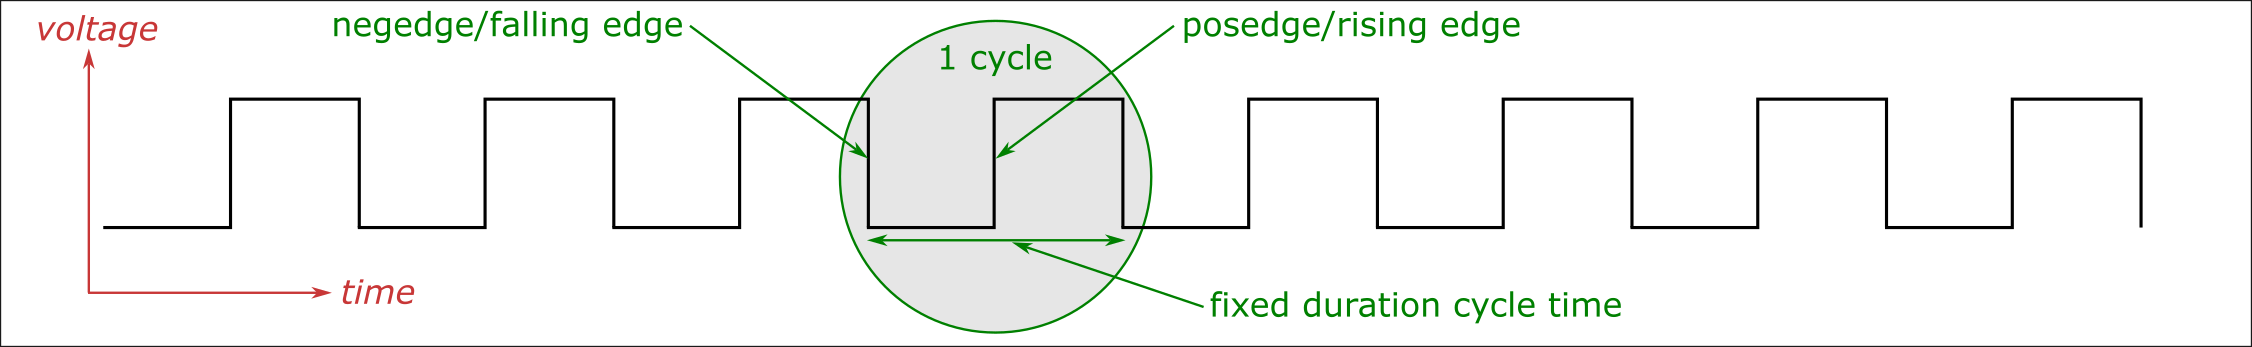
\includegraphics[width=\textwidth]{Fig_Clock}
\end{center}

\vspace{2ex}

The {\bsc} compiler tries to execute as many rules as possible in each
clock cycle (for maximum performance).

\vspace{2ex}

However, there are some constraints that limit this concurrency.

\end{frame}

% ================================================================

\begin{frame}[fragile]
\frametitle{Constraints on concurrent execution of rules in a clock (1/2)}

\footnotesize

Suppose we want to implement each rule in hardware as suggested in the
diagram in Slide~\ref{Slide_HW_representation_of_a_rule}.

\vspace{2ex}

Then, conceptually, at each posedge, all enabled rules (whose
CAN\_FIRE is true) will fire and perform their output actions.

\vspace{2ex}

But this would be wrong, for two reasons:

\begin{itemize}

 \item[(1)] Two rules may have \emph{Action Conflicts} or {\emph
       Resource Conflicts} if executed in the same clock.

       \vspace{2ex}

       Two rules may invoke the same {\tt Action}/{\tt ActionValue}
       method (write to the same register, or enqueue onto the same
       FIFO, dequeue the same FIFO, {\etc}).  This is clearly not
       feasible at the same instant (same clock posedge).

\end{itemize}

\end{frame}

% ================================================================

\begin{frame}[fragile]
\frametitle{Constraints on concurrent execution of rules in a clock (2/2)}

\footnotesize

\begin{itemize}

 \item[(2)] Two rules may have \emph{Ordering Conflicts} if executed
       in the same clock, {\ie} the \emph{ordering} can be
       inconsistent with rule semantics.

       \vspace{1ex}

       Consider these two rules, with {\tt x} and {\tt y} initially both having the value 10:

       \begin{center}
       \begin{minipage}{0.4\textwidth}
        {\footnotesize
        \begin{Verbatim}[frame=single]
rule rl_r1 (...);
   x <= y + 1;
endrule
        \end{Verbatim}
        }
       \end{minipage}
       \hmm
       \begin{minipage}{0.4\textwidth}
        {\footnotesize
        \begin{Verbatim}[frame=single]
rule rl_r2 (...);
   y <= x + 2;
endrule
        \end{Verbatim}
        }
       \end{minipage}
       \end{center}

       \vspace{1ex}

       According to the one-rule-at-a-time semantics,
       rule \verb|rl_r1| may precede \verb|rl_r2|. \\
       After \verb|rl_r1|, {\tt x} has the value 11.
       Then, after \verb|rl_r2|, {\tt y} has the value 13.

       \vspace{1ex}

       Or, according to the one-rule-at-a-time semantics,
       rule \verb|rl_r2| may precede \verb|rl_r1|. \\
       After \verb|rl_r2|, {\tt y} has the value 12.
       Then, after \verb|rl_r1|, {\tt x} has the value 13.

       \vspace{1ex}

       In either case, register state-update by one rule is observed
       by the other rule.

       \vspace{1ex}

       Whereas, if we execute both rules in the same clock (at the
       same instant), neither rule observes the update by the other
       rule. {\tt x} gets the value 11, and {\tt y} gets the value 12.
       This is inconsistent with the rule-at-a-time semantics, and
       therefore an incorrect execution.

\end{itemize}

\end{frame}

% ================================================================

\begin{frame}[fragile]
\frametitle{Rule arbitration and scheduling (1/2)}

\footnotesize

In summary, when two rules are enabled in the same clock and they have
any of the conflicts discussed above, one of them needs to
be \emph{stalled} for that clock.

\vspace{5ex}

Analogy:
\fbox{
\begin{minipage}{0.9\textwidth}

Managing rule conflicts is similar to managing \emph{write-write}
and \emph{read-write hazards} in processor pipelines, where
instruction I$_1$ writes to a register and the next instruction I$_2$
reads from that register---we may have to stall I$_2$ until I$_1$ has
performed its register-write.

\end{minipage}}

\end{frame}

% ================================================================

\begin{frame}[fragile]
\frametitle{Rule arbitration and scheduling (2/2)}

\footnotesize

Stalling a rule, when necessary, is performed by a \emph{rule
controller} (also sometimes called a \emph{scheduler}).

\begin{center}
 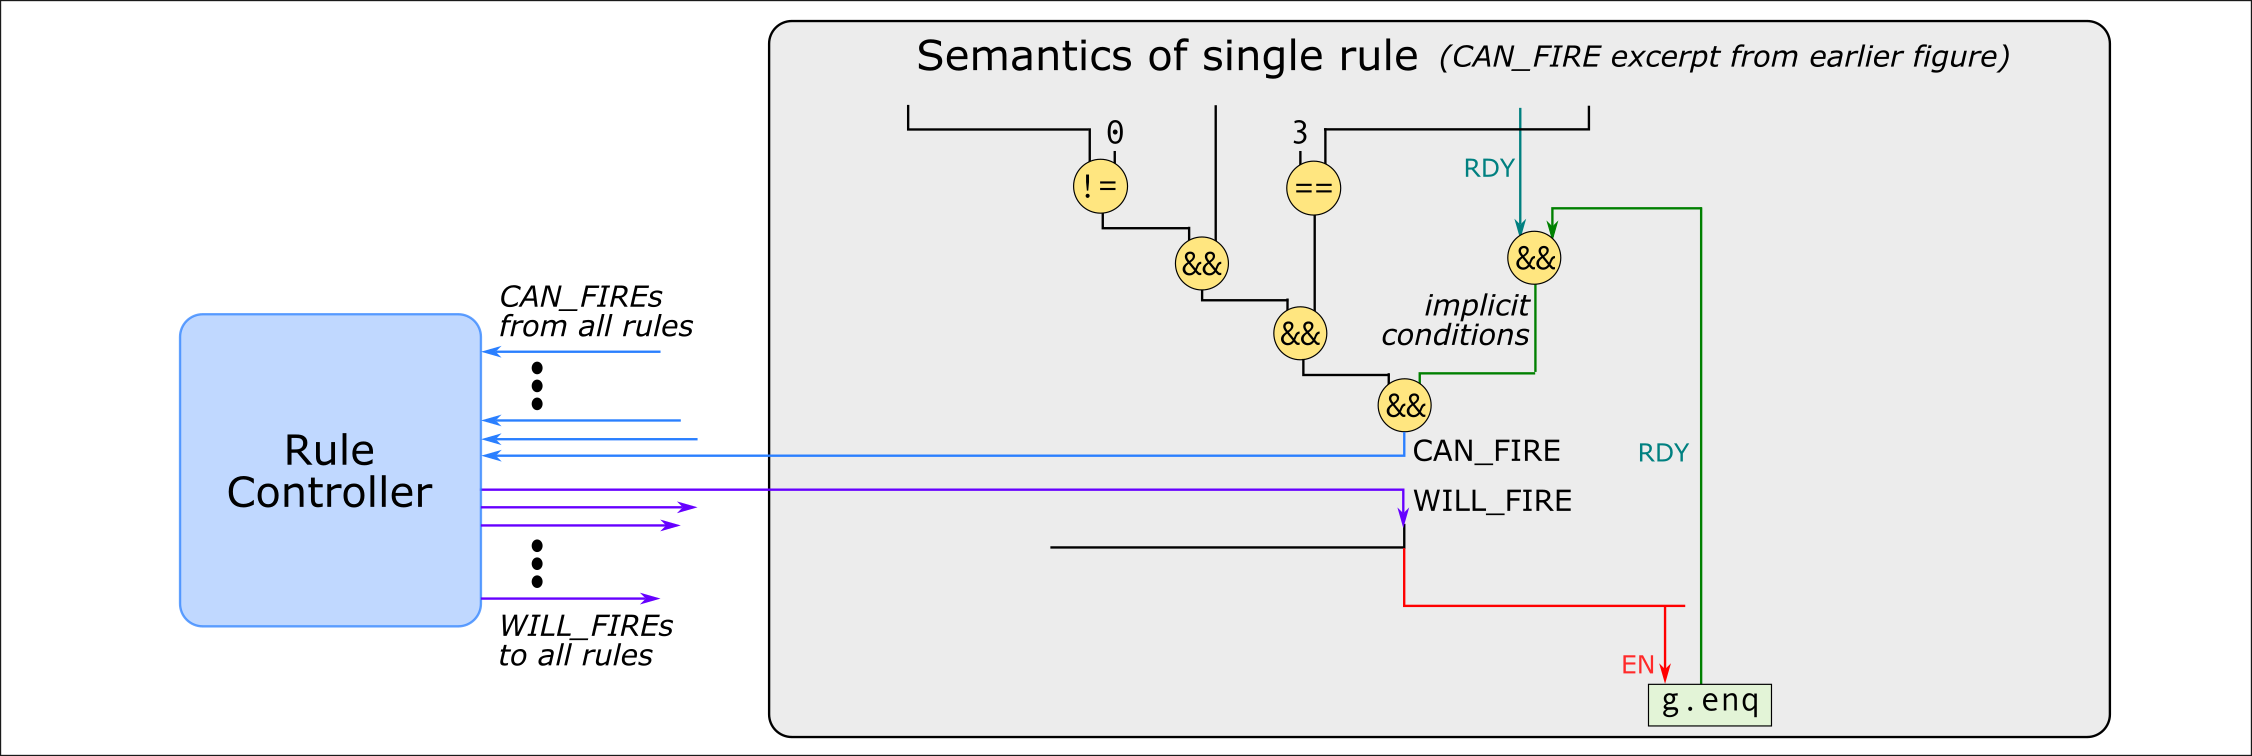
\includegraphics[width=0.9\textwidth]{Fig_Rule_Actions_Controlled}
\end{center}

This is a combinational circuit whose inputs are the {\tt CAN\_FIRE}
signals from all rules in the design.  For each {\tt CAN\_FIRE} input,
it has a corresponding {\tt WILL\_FIRE} output signal, which connects
to the ENABLE inputs of all the rule's actions.

\vspace{1ex}

The {\bsc} compiler designs a custom rule controller for each design,
based on an analysis of the actual rules in the design.  It ensures
that conflicting rules do not fire in the same clock.

\end{frame}

% ================================================================

\begin{frame}[fragile]
\frametitle{Guiding {\bsc}'s creation of the rule controller}

\footnotesize

When two rules with conflicts may both be enabled simultaneously (both
{\tt CAN\_FIRE}s true), the {\bsc} compiler uses various heuristics to
decide which one will be stalled by the generated rule controller.

\vspace{2ex}

\begin{minipage}{0.5\textwidth}
 {\bsc}'s choices are generally reasonable but, in rare cases, the
 programmer may wish to specify an explicit priority preference:
\end{minipage}
\hm
\begin{minipage}{0.45\textwidth}
\begin{Verbatim}[frame=single]
rule rl_r1 (...);
   ...
endrule

(* descending_urgency = "rl_r1, rl_r2" *)
rule rl_r2 (...);
   ...
endrule
\end{Verbatim}
\end{minipage}

\vspace{4ex}

\begin{minipage}{0.5\textwidth}
This attribute forces the rule controller to stall \verb|rl_r2|
whenever \verb|rl_r1| executes, whether or not they conflict:
\end{minipage}
\hm
\begin{minipage}{0.45\textwidth}
\begin{Verbatim}[frame=single]
(* preempts = "rl_r1, rl_r2" *)
\end{Verbatim}
\end{minipage}

\vspace{4ex}

\begin{minipage}{0.5\textwidth}
If two rules' {\tt CAN\_FIRE}s are mutually exclusive, they cannot
conflict; this permits more efficient rule controller hardware.
{\bsc} is quite good at recognizing mutual exclusivity automatically,
but the user can assist it explicitly:
\end{minipage}
\hm
\begin{minipage}{0.45\textwidth}
\begin{Verbatim}[frame=single]
(* mutually_exclusive = "rl_r1, rl_r2" *)
\end{Verbatim}
\end{minipage}

\end{frame}

% ****************************************************************

\section{Rules: Final Comments}

\begin{frame}

\begin{center}
  {\LARGE Rules: Final Comments}
\end{center}

\end{frame}

% ================================================================

\begin{frame}[fragile]
\frametitle{Rules: final comments}

\footnotesize

 \emph{Rules are a unique feature of {\BSV}. \\
       We are unaware of any other HDL (Hardware Description Language)
       where behavior is specified using rules.}

\vspace{2ex}

\begin{itemize}
 \item Rules are the fundamental (and only) behavioral construct in {\BSV}.

 \vspace{2ex}

 \item Each rule is an \emph{atomic transaction} modifying system
       state, which follows trivially from the rule-at-a-time
       semantics.

       \vspace{1ex}

       Atomicity is one of the most powerful concepts in Computer
       Science for reasoning about correctness of concurrent systems.

 \vspace{2ex}

 \item A rule comprises a syntactic {\tt rule}-{\tt endrule}
       construct; every interface method invoked by that rule; every
       method invoked by those methods; and so on.  The overall rule
       condition ({\tt CAN\_FIRE}) encompasses the rule's explicit
       condition and the implicit conditions of all those methods.

       \vspace{1ex}

       Thus, the atomicity of a rule is a \emph{non-local}
       property---through its methods, it may observe and update state
       across many modules.

 \vspace{2ex}

 \item The {\bsc} compiler compiles the rules in a design into clocked
       digital hardware, attempting to maximize concurrency (number of
       rules that can execute in a clock) while remaining consistent
       with the rule-at-a-time semantics.

\end{itemize}

\end{frame}

% ****************************************************************

\section{{\tt StmtFSM} is just an EDSL for Rules}

\begin{frame}

\begin{center}
  {\LARGE {\tt StmtFSM} is just an EDSL$^1$ for Rules}

  \vspace{20ex}

  {\footnotesize $^1$ Embedded Domain-Specific Language}
\end{center}

\end{frame}

% ================================================================

\begin{frame}[fragile]
\frametitle{{\tt StmtFSM} is just an EDSL for Rules (1/3)}

\footnotesize

Anything coded with {\tt StmtFSM} can also be coded explicitly using rules.  Example:

\begin{Verbatim}[frame=single]
   Stmt s = while (b)
               seq
	          action1;
	          if (c)
		     action2;
		  else
		     action3;
	          action4;
               endseq
\end{Verbatim}

\end{frame}

% ================================================================

\begin{frame}[fragile]
\frametitle{{\tt StmtFSM} is just an EDSL for Rules (2/3)}

\footnotesize

We can convert this into rules mechanically as follows:
\begin{itemize}
\item Each {\tt Action} in the {\tt Stmt} becomes the body of a rule.

\item We add a register {\tt rg\_step} to control the sequencing.  Each rule
      is enabled for a particu lar value of {\tt rg\_step}; when it
      executes, it updates {\tt rg\_step} to enable the next rule.

\end{itemize}

\begin{minipage}[t]{0.47\textwidth}
\begin{Verbatim}[frame=single]
   // rg_step == 7 means "idle"
   // To start the FSM,
   // environment sets rg_step <= 0
   Reg #(Bit #(3)) rg_step <- mkReg (7);

   rule rl_while (rg_step == 0);
      rg_step <= (b ? 1 : 100);
   endrule

   rule rl_A1 (rg_step == 1);
      action1;
      rg_step <= (c ? 2 : 3);  // if-then-else
   endrule
\end{Verbatim}
\end{minipage}
\begin{minipage}[t]{0.47\textwidth}
\begin{Verbatim}[frame=single]
   rule rl_A2 (rg_step == 2);
      action2;
      rg_step <= 4;
   endrule

   rule rl_A3 (rg_step == 3);
      action3;
      rg_step <= 4;
   endrule

   rule rl_A4 (rg_step == 4);
      action4;
      rg_step <= 0;    // back to top of loop
   endrule
\end{Verbatim}
\end{minipage}

\end{frame}

% ================================================================

\begin{frame}[fragile]
\frametitle{{\tt StmtFSM} is just an EDSL for Rules (3/3)}

\footnotesize

In summary, {\tt StmtFSM} is just an ``EDSL'' (Embedded
Domain-Specific Language) within {\BSV} for \emph{structured} rule
flows (rule flows that can be characterized as a composition of
sequencing, if-then-else, loops, and fork-join parallelism).

\vspace{5ex}

When we have \emph{unstructured} rule flows, {\tt StmtFSM} is not
appropriate, and we use rules directly ({\eg} in Fife).

\end{frame}

% ****************************************************************

% -*- mode: fundamental -*-

% Slides accompanying "Learn RISC-V CPU Implementation and BSV" book
% Copyright (c) 2024 Rishiyur S. Nikhil, All Rights Reserved

% This is a postamble shared by all the slide decks

% ================================================================

\begin{frame}

\begin{center}
  {\LARGE End}
\end{center}

\end{frame}

% ================================================================


% ****************************************************************

\end{document}
% ****************************************************************
